\section{Экспериментально-исследовательская часть}

В данном разделе будет проведено исследование влияния кеширования на производительность разработанного ПО.

\subsection{Цель проводимых измерений}

Основным сценарием использования разработанного веб-сервера является сохранение терминов после обработки текстов. Это означает, что серверу будут поступать запросы на запись данных, объёмы которых могут превышать объёмы исходных текстов. Чтобы ускорить обработку данных и повысить отзывчивость приложения, можно применить кеширование, то есть запись данных в промежуточное хранилище в оперативной памяти сервера. Далее данные могут быть перемещены в долговременное хранилище.

Целью проводимых измерений будет проведение нагрузочного тестирования и сравнение производительности веб-сервера при обработке запросов на сохранение терминов с использованием кеширования и без него.


	
\subsection{Описание проводимых измерений}

Для исследования в приложении был реализован компонент доступа к данным, работающий с Redis. Он предназначен для того, чтобы избежать обращения к долговременному хранилищу (PostgreSQL). Это позволит сократить время выполнения запроса на сохранение терминов. Конфигурация запуска Redis представлена в приложении Е.

Для тестирования была выбрана конечная точка /api/v1/units, через которую осуществляется сохранение терминов. 

Для проведения нагрузочного тестирования необходимо выбрать модель нагрузки: открытую или закрытую.

% RPS
При тестировании с открытой моделью нагрузки количество пользователей системы неисчислимо. Интенсивность нагрузки не зависит от состояния тестируемого сервиса и скорости его ответа на запросы. % (до определенного ощутимого предела)
С увеличением времени ответа нагрузка на сервис растёт, а значит растёт и количество параллельно обрабатываемых запросов.
Для тестирования необходимо задать RPS, то есть количество одновременных запросов к приложению в секунду.

% Открытая модель — на графике могут быть видны пики и провалы, и это нормально для этой модели. Пик на графике должен коррелировать с увлечением времени отклика, так как в этот момент пользователи ожидают ответа от сервера и общая нагрузка на систему начинает падать. В связи с чем инструмент начинает поднимать новых виртуальных пользователей, чтобы количество запросов к системе оставалось постоянным, несмотря на долгие ответы/ошибки приложения. Для защиты от чрезмерного увеличения количества пользователей необходимо использовать функции троттлинга, принудительно задающие верхний порог — максимальное количество поднятых пользователей инструментом нагрузки.

% Instances
Для тестирования с закрытой моделью нагрузки заранее задаётся число пользователей системы, которые посылают запросы в систему без задержек. Интенсивность нагрузки зависит от того, как быстро отвечает сервис. И чем быстрее отвечает тестируемый сервис, тем большую нагрузку создают пользователи. 

% Это создает эффект, при котором деградация тестируемой системы влечет за собой уменьшение потока запросов (при неизменном количестве соединений).

% И процесс, который происходит в течение работы сервиса, подчиняется множеству пользователей, использующих его. Говоря проще, чем медленнее отвечает сервис, тем меньшую нагрузку пользователи создают (в запросах в секунду). Для того, чтобы визуально представить как это работает, вспомните любой гипермаркет и представьте, что это наш сервис. Кассы в данном случае - это обработчики клиентов, их количество ограничено. Чем медленнее они будут работать, тем меньше клиентов через них пройдёт. Их производительность ограничена временем работы, а нагрузка на условный сервис - количеством касс.

% Закрытая модель — пользователи должны заходить в систему согласно планируемому профилю нагрузки. Если на графике видны провалы или пики, это говорит о том, что нагрузка шла не по рассчитанному или запланированному сценарию, и требует дальнейшего изучения

При тестировании будут использоваться обе модели нагрузки: открытая модель нагрузки позволит сымитировать поведение пользователей веб-сервиса, а закрытая позволит определить время, за которое система выполнит заданный объём работы.



\subsection{Инструменты измерения времени обработки запросов}

Для проведения нагрузочного тестирования использовался инструмент оценки нагрузки и производительности Yandex.Tank \cite{yandex_tank}. Для визуализации результатов нагрузочного тестирования использовался сервис для мониторинга и анализа нагрузочного тестирования Overload \cite{overload}. В качестве генератора нагрузки использовался Phantom \cite{phantom}.

% Он позволяет анализировать приложение под нагрузкой, визуализируя результаты в виде графиков.

Для проведения нагрузочного тестирования с помощью Yandex.Tank было выбрано три профиля нагрузки:

\begin{enumerate}[label*=\arabic*)]
	\item открытая линейная --- от 1 до 25 rps на протяжении 3 минут;
	\item открытая постоянная --- 20 rps на протяжении 1 минуты;
	\item закрытая --- 1 пользователь последовательно посылает 10000 запросов.
\end{enumerate}

В листингах \ref{lst:conf1}-\ref{lst:conf3} представлена конфигурация для проведения нагрузочного тестирования с помощью Yandex.Tank.

\lstinputlisting[label=lst:conf1, caption={Конфигурация для тестирования с открытой линейной нагрузкой}]{../../yandex_tank/line_load_rps.yaml}

\lstinputlisting[label=lst:conf2, caption={Конфигурация для тестирования с открытой постоянной нагрузкой}]{../../yandex_tank/const_load_rps.yaml}

\lstinputlisting[label=lst:conf3, caption={Конфигурация для тестирования с закрытой нагрузкой}]{../../yandex_tank/const_load_instances.yaml}

В листинге \ref{lst:conf4} представлен HTTP-запрос, использовавшийся для тестирования.

\lstinputlisting[label=lst:conf4, caption={HTTP-запрос для тестирования}]{../../yandex_tank/ammo.txt}



\subsection{Технические характеристики оборудования}

Ниже приведены технические характеристики устройства, на котором выполнялось тестирование.

\begin{itemize}[label*=---]
	\item Операционная система: Manjaro Linux x86\_64 \cite{manjaro}, версия ядра 5.15.32.
	\item Объём оперативной памяти: 16 Гб.
	\item Процессор: Intel i5-9300H 2.4 ГГц \cite{intel}.
\end{itemize}

Тестирование проводилось на ноутбуке, включенном в сеть электропитания. Во время тестирования ноутбук был нагружен только встроенными приложениями окружения, а также непосредственно системой тестирования.


		
\subsection{Результаты проведённых измерений}

Ниже представлены результаты нагрузочного тестирования разработанного приложения, оформленные в виде графиков зависимости времени ответа веб-сервера от времени и RPS, создаваемого генератором нагрузки. На графиках показана зависимость от времени работы сервиса следующих метрик:

\begin{enumerate}[label*=\arabic*)]
	\item RPS;
	\item среднее время ответа веб-сервера (avg, average);
	\item квантиль уровня 98\% времени ответа --- промежуток времени, за который веб-сервер отвечает на 98\% запросов.
\end{enumerate}

% Квантиль* уровня n – время, в которое укладывается n% ответов

\subsubsection{Открытая линейная нагрузка}

На рисунках \ref{fig:line_load_rps_nocached} и \ref{fig:line_load_rps_cached} представлены результаты проведения нагрузочного тестирования при открытой линейной нагрузке с использованием и без использования кеширования.

\begin{figure}[h]
	\centering
	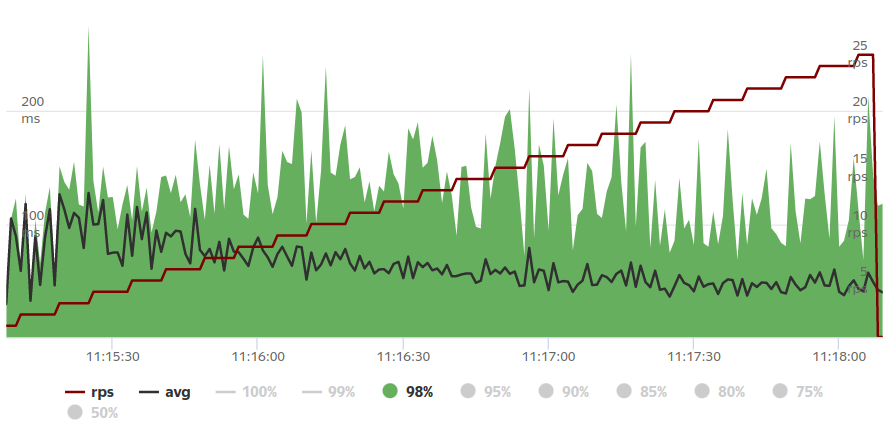
\includegraphics[width=\textwidth ]{img/Load_testing/line_load_rps_nocached.png}
	\caption{Результат проведения нагрузочного тестирования при открытой линейной нагрузке без использования кеширования}
	\label{fig:line_load_rps_nocached}
	
	\centering
	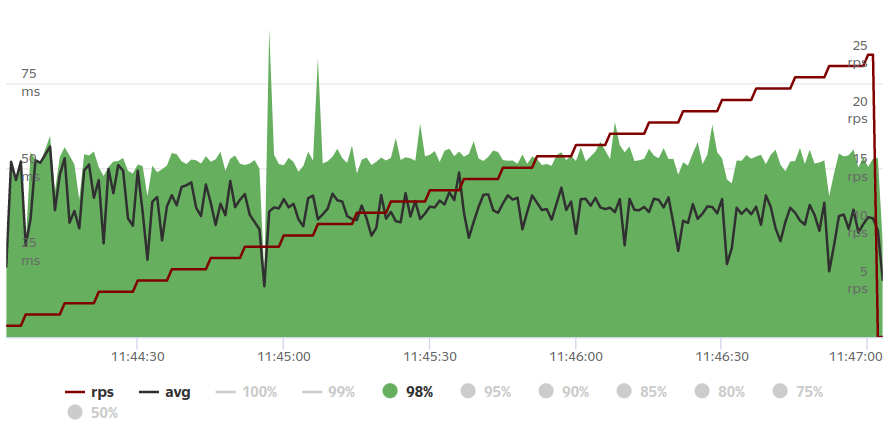
\includegraphics[width=\textwidth ]{img/Load_testing/line_load_rps_cached.png}
	\caption{Результат проведения нагрузочного тестирования при открытой линейной нагрузке с использованием кеширования}
	\label{fig:line_load_rps_cached}
\end{figure} 

\clearpage

При использовании кеширования среднее время ответа сервера уменьшилось с 63 мс до 37 мс. Также уменьшился разброс времён ответов, то есть сервер стал отвечать на запросы стабильнее. % (потому что стало меньше скачков и квантиль уровня 98% приблизилась к avg)

\subsubsection{Открытая постоянная нагрузка}

На рисунках \ref{fig:const_load_rps_nocached} и \ref{fig:const_load_rps_cached} представлены результаты проведения нагрузочного тестирования при открытой постоянной нагрузке с использованием и без использования кеширования.

\begin{figure}[h]
	\centering
	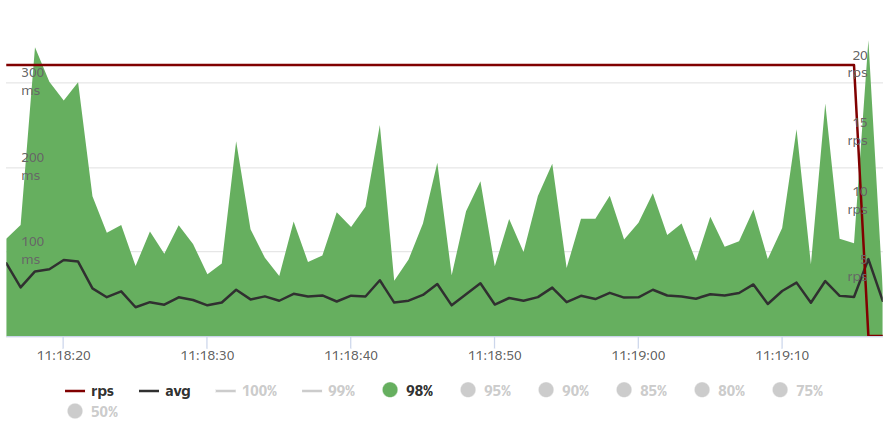
\includegraphics[width=\textwidth ]{img/Load_testing/const_load_rps_nocached.png}
	\caption{Результат проведения нагрузочного тестирования при открытой постоянной нагрузке без использования кеширования}
	\label{fig:const_load_rps_nocached}
	
	\centering
	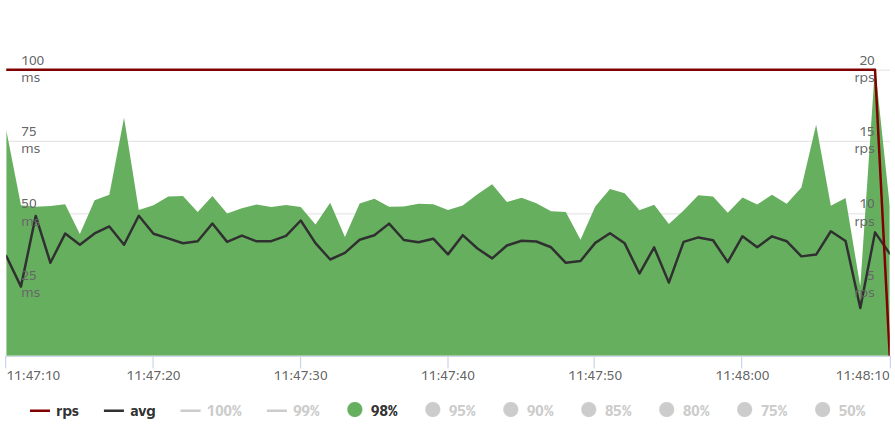
\includegraphics[width=\textwidth ]{img/Load_testing/const_load_rps_cached.png}
	\caption{Результат проведения нагрузочного тестирования при открытой постоянной нагрузке с использованием кеширования}
	\label{fig:const_load_rps_cached}
\end{figure} 

\clearpage

При использовании кеширования среднее время ответа сервера уменьшилось с 49 мс до 38 мс. Также уменьшился разброс времён ответов, то есть сервер стал отвечать на запросы стабильнее. % (потому что стало меньше скачков и квантиль уровня 98% приблизилась к avg)

\subsubsection{Закрытая нагрузка}

На рисунках \ref{fig:const_load_instances_nocached} и \ref{fig:const_load_instances_cached} представлены результаты проведения нагрузочного тестирования при закрытой нагрузке с использованием и без использования кеширования.

\begin{figure}[h]
	\centering
	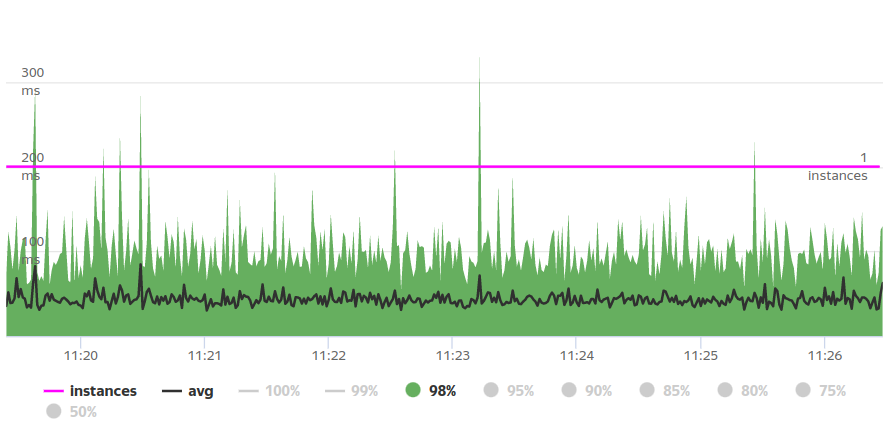
\includegraphics[width=\textwidth ]{img/Load_testing/const_load_instances_nocached.png}
	\caption{Результат проведения нагрузочного тестирования при закрытой нагрузке без использования кеширования}
	\label{fig:const_load_instances_nocached}
	
	\centering
	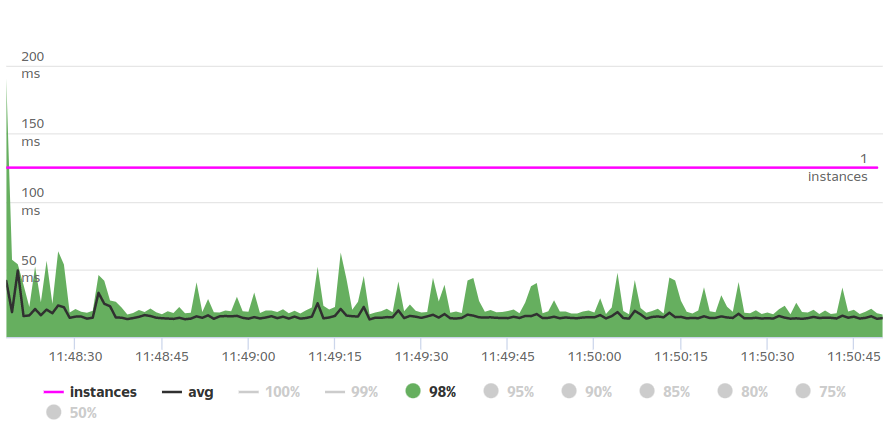
\includegraphics[width=\textwidth ]{img/Load_testing/const_load_instances_cached.png}
	\caption{Результат проведения нагрузочного тестирования при закрытой нагрузке с использованием кеширования}
	\label{fig:const_load_instances_cached}
\end{figure} 

\clearpage

При использовании кеширования среднее время ответа сервера уменьшилось с 44 мс до 15 мс. Также уменьшился разброс времён ответов, то есть сервер стал отвечать на запросы стабильнее. % (потому что стало меньше скачков и квантиль уровня 98% приблизилась к avg)
Суммарное время обработки 10000 запросов от 1 пользователя уменьшилось с 6 минут 53 секунд до 2 минут 17 секунд, то есть на 66\%.



\subsection*{Вывод из экспериментально-исследовательской части}

% По графикам сделать выводы об удачности эксперимента по внедрению кеширования в работу приложения.

% Исследовать влияние использования кеширования данных на время обработки запросов к приложению. 

В данном разделе было проведено исследование влияния кеширования на производительность разработанного ПО.

Измерения показали, что кеширование позволило повысить производительность веб-сервера, а именно его конечной точки /api/v1/units. При тестировании с использованием открытой модели нагрузки среднее время ответа сервера уменьшилось на 41\% при линейной нагрузке и 22\% при постоянной нагрузке. При тестировании с использованием закрытой модели нагрузки среднее время ответа сервера уменьшилось на 66\%. Также использование кеширования позволило устранить пиковые нагрузки на сервис и сделать его работу более стабильной.



\pagebreak